\documentclass[11pt,a4paper]{article}

% ============================================================
% Packages
% ============================================================
\usepackage[margin=1in]{geometry}
\usepackage[utf8]{inputenc}
\usepackage[T1]{fontenc}
\usepackage{times}            % Times New Roman font
\usepackage{amsmath,amssymb}
\usepackage{graphicx}
\usepackage{booktabs}
\usepackage{hyperref}
\usepackage{xcolor}
\usepackage{enumitem}
\usepackage{caption}
\usepackage{float}
\usepackage{microtype}
\usepackage{natbib}
\usepackage{url}
\usepackage{titlesec}

% Compact spacing
\usepackage{setspace}
\setstretch{1.0}
\setlength{\parskip}{2pt plus 1pt minus 1pt}
\setlength{\parindent}{1em}

% Compact section titles
\titlespacing*{\section}{0pt}{10pt plus 2pt minus 2pt}{4pt plus 1pt minus 1pt}
\titlespacing*{\subsection}{0pt}{8pt plus 2pt minus 2pt}{3pt plus 1pt minus 1pt}

\hypersetup{
    colorlinks=true,
    linkcolor=blue!70!black,
    citecolor=blue!70!black,
    urlcolor=blue!70!black,
}

\graphicspath{{figures/}}

% ============================================================
\begin{document}

% ============================================================
% Title
% ============================================================
\begin{center}
    {\Large\bfseries MedBot: Domain-Specific Retrieval-Augmented Generation\\[4pt]
    for Medical Question Answering}\\[12pt]
    {\normalsize C.~Cai\quad Y.~Liao\quad D.~Liu\quad Y.~Qian\quad Y.~Huang\quad Y.~Wang}\\[4pt]
    {\small MH6812 Natural Language Processing --- Nanyang Technological University}\\[4pt]
    {\footnotesize\texttt{\{CHUYUE002, YUQING011, DONGYANG002, YICHEN009, YAQUN001, WANG2322\}@e.ntu.edu.sg}}
\end{center}

\vspace{6pt}

% ============================================================
% Abstract
% ============================================================
\begin{abstract}
Large language models frequently hallucinate on medical queries, generating plausible but unsupported claims that pose risks in health-related settings. We present MedBot, a retrieval-augmented generation (RAG) system for medical question answering that grounds responses in domain-specific evidence. MedBot uses PubMedBERT-based sentence embeddings for semantic retrieval over four medical knowledge bases (70,000+ documents), combined with a confidence-scoring mechanism that triggers cross-collection fallback when retrieval quality is low. Structured prompt engineering further constrains the LLM to cite retrieved evidence and acknowledge uncertainty. In our evaluation, PubMedBERT embeddings outperform general-purpose MiniLM by +0.37 mean cosine similarity on medical synonym pairs, the retrieval pipeline achieves Recall@3 of 94.7\% and MRR of 0.906 across 300 test queries on the full 70K+ corpus, and the confidence scoring mechanism correctly identifies out-of-domain queries to prevent hallucination.
\end{abstract}

% ============================================================
\section{Introduction}
% ============================================================

The application of natural language processing (NLP) to the medical domain presents a unique constellation of challenges. Medical text is characterized by highly specialized terminology, complex semantic relationships between diseases, symptoms, and treatments, and a significant vocabulary gap between clinical professionals and lay users~\citep{gu2021domain}. A patient searching for information about ``chest tightness'' must be matched to documents discussing ``angina pectoris'' or ``dyspnea,'' requiring models that understand deep semantic equivalences rather than surface-level lexical overlap. Moreover, the stakes of medical information systems are exceptionally high: inaccurate or fabricated medical advice can lead to delayed treatment, inappropriate self-medication, or unnecessary anxiety~\citep{jin2021disease}.

General-purpose large language models such as GPT-5 and DeepSeek have achieved impressive performance across many NLP benchmarks, yet they frequently hallucinate---generating fluent but factually incorrect statements. In the medical domain, fabricated drug interactions or clinical statistics can directly harm patients. Fine-tuning LLMs on medical corpora partially addresses this, but requires substantial computational resources and cannot easily incorporate new evidence.

Retrieval-augmented generation (RAG) offers a compelling alternative by decoupling the knowledge source from the generation model~\citep{lewis2020retrieval}. Rather than relying on parametric knowledge, RAG systems retrieve relevant passages from an external knowledge base at inference time. This provides three advantages for medical QA: (1)~responses are grounded in verifiable sources; (2)~the knowledge base can be updated without retraining; and (3)~retrieval confidence can be quantified and communicated to the user.

This paper presents MedBot, a domain-specific RAG system for medical question answering. The system uses a PubMedBERT-based embedding model (\texttt{S-PubMedBert-MS-MARCO}) to encode queries and documents into a shared 768-dimensional space, retrieves evidence from four medical knowledge bases totaling 70K+ documents~\citep{abacha2019question,jin2019pubmedqa,jin2021disease} via ChromaDB, applies confidence scoring with cross-collection fallback when retrieval quality is low, and constrains generation through structured prompts that enforce evidence citation and uncertainty acknowledgment.

In our evaluation, PubMedBERT embeddings outperform MiniLM-L6-v2 by +0.37 cosine similarity on medical synonyms, and the retrieval pipeline achieves Recall@3 of 94.7\% and MRR of 0.906 across 300 test queries on the full corpus.

% ============================================================
\section{Related Work}
% ============================================================

\subsection{Pretrained Language Models for Biomedical NLP}

BioBERT~\citep{lee2020biobert} demonstrated that continued pretraining of BERT on PubMed abstracts improves biomedical NER, relation extraction, and QA. \citet{gu2021domain} further showed that pretraining from scratch on PubMed alone (PubMedBERT) outperforms mixed-domain models, arguing that domain-specific vocabulary matters more than model size. These findings motivate our choice of PubMedBERT.

\subsection{Retrieval-Augmented Generation}

Retrieval-augmented generation was formalized by \citet{lewis2020retrieval}, who proposed combining a pretrained retriever with a sequence-to-sequence generator. The REALM framework~\citep{guu2020retrieval} introduced joint pretraining of the retriever and language model, treating the knowledge base as a latent variable. Dense Passage Retrieval (DPR)~\citep{karpukhin2020dense} demonstrated that learned dense representations substantially outperform BM25 for open-domain QA. More recent work has explored hybrid retrieval strategies combining lexical and semantic signals via Reciprocal Rank Fusion (RRF). Our system builds on these foundations by employing dense retrieval with domain-specific embeddings and incorporating confidence scoring to modulate the generation process.

\subsection{Medical QA Benchmarks and Sentence Transformers}

Several benchmarks evaluate medical QA: MedQA~\citep{jin2021disease} provides licensing exam questions, PubMedQA~\citep{jin2019pubmedqa} uses PubMed abstracts, BioASQ~\citep{treccovid2020} organizes annual evaluations, and MedQuAD~\citep{abacha2019question} aggregates NIH Q\&A pairs. These serve dual roles in our work as knowledge bases and evaluation benchmarks. For efficient sentence-level similarity, Sentence-BERT~\citep{reimers2019sentence} uses siamese BERT networks. MedBot's embedding model combines PubMedBERT domain pretraining with MS-MARCO retrieval fine-tuning.

% ============================================================
\section{Approach}
% ============================================================

The MedBot system comprises six principal components: a domain-specific embedding model, a vector retrieval engine, a confidence scoring mechanism, a cross-collection fallback strategy, a prompt engineering framework, and bilingual language support. Figure~\ref{fig:architecture} illustrates the overall system architecture.

\begin{figure}[t]
    \centering
    
\includegraphics[width=0.88\columnwidth]{architecture.png}
    \caption{System architecture of the MedBot RAG pipeline. User queries are encoded by PubMedBERT, matched against ChromaDB collections, scored for confidence, and passed to the LLM for grounded response generation.}
    \label{fig:architecture}
\end{figure}

\subsection{Embedding Model}

The embedding backbone is S-PubMedBERT (\texttt{pritamdeka/S-PubMedBert-MS-MARCO}), a domain-adapted Sentence-BERT model. The base architecture is PubMedBERT~\citep{gu2021domain}, a BERT variant~\citep{devlin2019bert} pre-trained exclusively on biomedical literature from PubMed abstracts and PubMed Central full-text articles. This 12-layer Transformer~\citep{vaswani2017attention} encoder produces 768-dimensional dense embeddings and contains approximately 110 million parameters. The model was subsequently fine-tuned on the MS-MARCO passage ranking dataset, which aligns query and relevant passage representations in the shared embedding space for retrieval tasks.

\subsection{Vector Retrieval}

MedBot employs ChromaDB as its persistent vector database, storing all document embeddings as 768-dimensional vectors indexed with the L2 (Euclidean) distance metric. At query time, the user's input is encoded by S-PubMedBERT and a nearest-neighbor search retrieves the top-$K=8$ most similar document chunks from the target collection.

\subsection{Confidence Scoring}

A critical requirement for medical QA is the ability to recognize when retrieved evidence is insufficient. MedBot converts raw retrieval distances into an interpretable confidence score on $[0,1]$. Given the set of L2 distances, the system computes a combined distance:
\begin{equation}
    d_{\text{combined}} = 0.6 \times d_{\min} + 0.4 \times d_{\text{avg}}
\end{equation}
This combined distance is mapped to a confidence score:
\begin{equation}
    \text{confidence} = \max\!\Big(0,\; \min\!\Big(1,\; \frac{50 - d_{\text{combined}}}{30}\Big)\Big)
\end{equation}
The weighting scheme emphasizes the closest match ($d_{\min}$) while penalizing retrievals where only a single result is close. The confidence score is mapped to four discrete levels (Table~\ref{tab:confidence}).

\begin{table}[t]
\centering
\caption{Confidence levels and corresponding system actions.}
\label{tab:confidence}
\begin{tabular}{@{}lcc@{}}
\toprule
\textbf{Level} & \textbf{Threshold} & \textbf{System Action} \\
\midrule
High     & $\geq 0.75$ & Return response directly \\
Medium   & $\geq 0.55$ & Return with advisory note \\
Low      & $\geq 0.30$ & Cross-collection fallback \\
Very Low & $< 0.30$    & Fallback + disclaimer \\
\bottomrule
\end{tabular}
\end{table}

\subsection{Cross-Collection Fallback}

When the primary collection yields low confidence, MedBot searches all four knowledge bases. The fallback retrieves top-$K$ candidates from each collection independently, merges results, sorts by L2 distance, and selects the overall top-$K$ documents. Fallback results are only adopted if they produce higher confidence than the primary retrieval, preventing degradation on irrelevant queries.

\subsection{Prompt Engineering}

The generation component uses a structured prompt template enforcing a tiered response structure: acknowledge symptoms, provide differential diagnosis, then stratify guidance into home care, indicators for professional attention, and emergency warning signs. All responses must cite retrieved source documents. Safety guardrails instruct the model to refrain from definitive diagnoses and recommend professional consultation for serious symptoms.

\subsection{Bilingual Support}

Since the embedding model and knowledge bases are English-only, MedBot translates Chinese input to English for retrieval, then generates responses in the user's detected language. This preserves retrieval quality while extending accessibility to Chinese-speaking users.

% ============================================================
\section{Experiments}
% ============================================================

We present four experiments evaluating embedding quality, retrieval accuracy, confidence scoring effectiveness, and full pipeline behavior.

\subsection{Data}

MedBot draws on four publicly available medical datasets (Table~\ref{tab:data}). The combined corpus contains 70,835 source documents. During preprocessing, documents are split into chunks of at most 800 characters with 100-character overlap, using sentence boundary splitting (minimum 50, maximum 2,000 characters per chunk).

\begin{table}[t]
\centering
\caption{Summary of knowledge base datasets.}
\label{tab:data}
\begin{tabular}{@{}lrll@{}}
\toprule
\textbf{Dataset} & \textbf{Documents} & \textbf{Source} & \textbf{Content} \\
\midrule
MedQuAD         & 35,087 & NIH         & Symptom Q\&A pairs \\
FDA Drug Labels & 1,804  & OpenFDA API & Medication information \\
PubMedQA        & 14,400 & PubMed      & Biomedical Q\&A \\
MedQA           & 19,544 & USMLE exams & Medical exam Q\&A \\
\bottomrule
\end{tabular}
\end{table}

\subsection{Model Settings}

All experiments use the S-PubMedBERT embedding model (\texttt{pritamdeka/\allowbreak S-PubMedBert-MS-MARCO}, 110M parameters, 768-dim output). Documents are chunked at 800 characters with 100-character overlap. ChromaDB uses L2 distance with top-$K{=}8$ retrieval. Confidence thresholds are set to 0.75 (high), 0.55 (medium), and 0.30 (low). For response generation, we use the OpenAI API (GPT-5.2) as the primary LLM provider, with DeepSeek-Chat as a fallback, and a maximum output length of 1,024 tokens. All embeddings are computed on a single GPU; retrieval and generation run at inference time with no additional training.

\subsection{Evaluation Metrics}

We adopt standard information retrieval metrics. \textbf{Recall@$K$} ($K \in \{1,3,5,10\}$) measures the fraction of queries with a relevant document in the top-$K$ results. \textbf{Mean Reciprocal Rank (MRR)} computes the average of $1/\text{rank}$ for the first relevant result. For embedding quality, we use \textbf{cosine similarity} between medical synonym embeddings.

\subsection{Experiment 1: Domain-Specific vs.\ General Embeddings}

We compare S-PubMedBERT against MiniLM-L6-v2, a general-purpose sentence embedding model, on six medical synonym pairs (lay term vs.\ clinical equivalent). Table~\ref{tab:embedding} presents the results.

\begin{table}[t]
\centering
\caption{Cosine similarity on medical synonym pairs.}
\label{tab:embedding}
\begin{tabular}{@{}llccc@{}}
\toprule
\textbf{Lay Term} & \textbf{Clinical Term} & \textbf{PubMed} & \textbf{MiniLM} & \textbf{$\Delta$} \\
\midrule
chest pain       & myocardial infarction  & 0.866 & 0.355 & +0.511 \\
headache         & cephalgia              & 0.893 & 0.395 & +0.498 \\
high blood sugar & hyperglycemia          & 0.934 & 0.629 & +0.305 \\
feeling sad      & major depressive disorder & 0.876 & 0.479 & +0.397 \\
stomach ache     & gastritis              & 0.906 & 0.570 & +0.336 \\
high blood pressure & hypertension        & 0.944 & 0.748 & +0.196 \\
\midrule
\textbf{Mean}    &                        & \textbf{0.903} & \textbf{0.529} & \textbf{+0.373} \\
\bottomrule
\end{tabular}
\end{table}

S-PubMedBERT achieves a mean cosine similarity of 0.903, compared to 0.529 for MiniLM (+0.373). The advantage is most pronounced where lay and clinical terms share no lexical overlap, such as ``chest pain'' vs.\ ``myocardial infarction'' (+0.511). This confirms that domain-specific pre-training captures medical synonym relationships that general-purpose models miss (Figure~\ref{fig:model_comparison}).

\begin{figure}[t]
    \centering
    
\includegraphics[width=0.88\columnwidth]{model_comparison.png}
    \caption{Cosine similarity comparison between PubMedBERT and MiniLM on medical synonym pairs.}
    \label{fig:model_comparison}
\end{figure}

\subsection{Experiment 2: Retrieval Quality}

We evaluate retrieval over the full 70K+ document corpus using 300 known-item queries drawn from two complementary test sets:

\textbf{Test Set~A: PubMedQA Known-Item Retrieval} (200 queries). We sample 200 unique labeled PubMedQA entries and use each entry's research question as the query. The ground truth is any document chunk sharing the same PubMed ID (PMID). Retrieval is performed against the full \texttt{pubmedqa} collection (14,400 documents).

\textbf{Test Set~B: MedQuAD Condition Retrieval} (100 queries). We sample 100 unique medical condition names from MedQuAD and use each condition name as the query. The ground truth is any chunk with a matching \texttt{condition} field. Retrieval is performed against the full \texttt{medquad\_symptoms} collection (35,087 documents).

Table~\ref{tab:retrieval} presents per-collection and aggregate results.

\begin{table}[t]
\centering
\caption{Retrieval evaluation results across 300 test queries on the full corpus.}
\label{tab:retrieval}
\begin{tabular}{@{}lccc@{}}
\toprule
\textbf{Metric} & \textbf{PubMedQA} & \textbf{MedQuAD} & \textbf{Aggregate} \\
 & (n=200) & (n=100) & (n=300) \\
\midrule
Recall@1  & 98.5\% & 65.0\% & 87.3\% \\
Recall@3  & 99.5\% & 85.0\% & 94.7\% \\
Recall@5  & 99.5\% & 86.0\% & 95.0\% \\
Recall@10 & 99.5\% & 87.0\% & 95.3\% \\
MRR       & 0.990  & 0.738  & 0.906 \\
\bottomrule
\end{tabular}
\end{table}

PubMedQA retrieval is near-perfect (Recall@1 = 98.5\%, MRR = 0.990), which is expected since the questions were authored to match their corresponding PubMed abstracts. MedQuAD condition retrieval is more challenging: querying by condition name against a 35K-document corpus yields Recall@1 of 65.0\% and Recall@3 of 85.0\%, reflecting the vocabulary diversity of medical conditions and the fact that condition names alone may not match the full Q\&A text semantically. In aggregate across all 300 queries, the system achieves Recall@3 of 94.7\% and MRR of 0.906 (Figure~\ref{fig:retrieval_metrics}).

\begin{figure}[t]
    \centering
    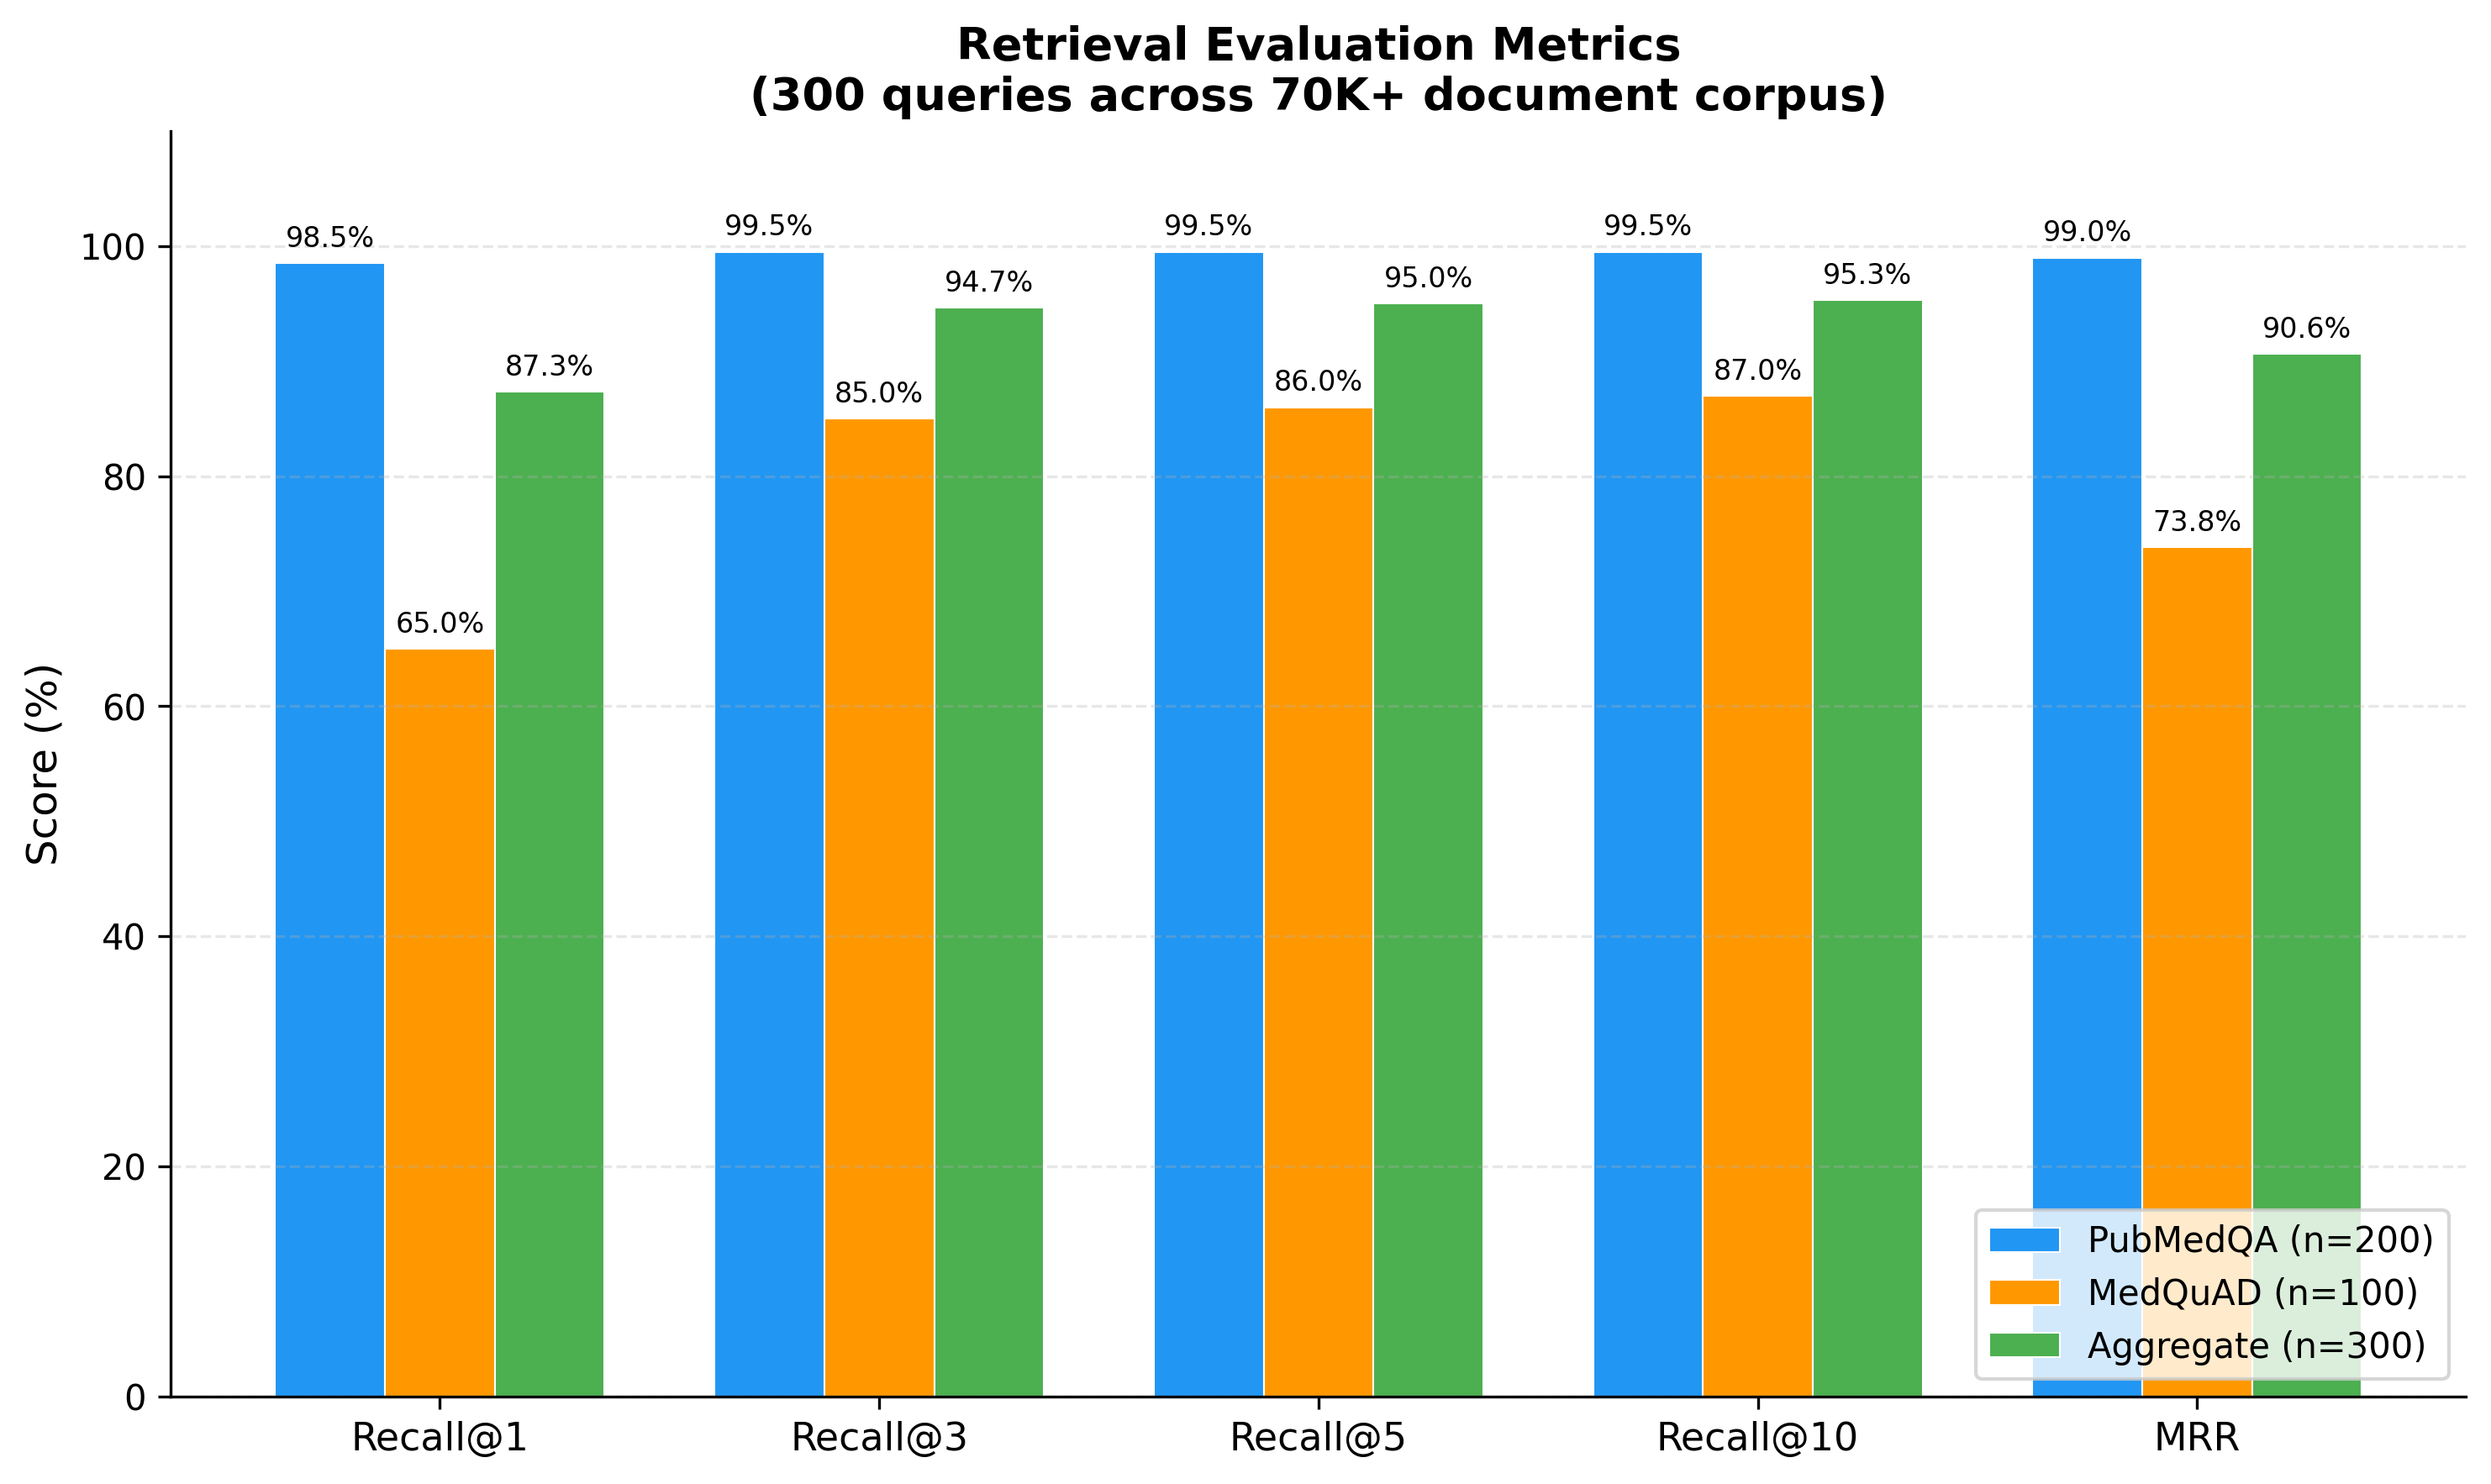
\includegraphics[width=0.88\columnwidth]{retrieval_metrics.png}
    \caption{Retrieval evaluation metrics across 300 queries on the full 70K+ document corpus. Per-collection and aggregate Recall@$K$ and MRR are shown.}
    \label{fig:retrieval_metrics}
\end{figure}

\subsection{Experiment 3: Confidence Scoring Effectiveness}

We test three queries of varying medical relevance (Table~\ref{tab:confidence_results}).

\begin{table}[t]
\centering
\caption{Confidence scoring results across query types.}
\label{tab:confidence_results}
\begin{tabular}{@{}lccl@{}}
\toprule
\textbf{Query} & \textbf{Conf.} & \textbf{Level} & \textbf{Category} \\
\midrule
``severe headache and nausea'' & 0.607 & Medium & In-domain \\
``chest hurts when I breathe'' & 0.395 & Low    & Related \\
``quantum physics experiments'' & 0.000 & Very Low & Out-of-domain \\
\bottomrule
\end{tabular}
\end{table}

The in-domain query receives medium confidence (0.607), triggering the standard response with an advisory note. The related medical query receives low confidence (0.395), activating cross-collection fallback. The out-of-domain query receives zero confidence, causing the system to issue a disclaimer. This graduated response demonstrates effective modulation of system behavior (Figure~\ref{fig:confidence}).

\begin{figure}[t]
    \centering
    
\includegraphics[width=0.88\columnwidth]{confidence_scoring.png}
    \caption{Confidence scoring across query types with threshold lines.}
    \label{fig:confidence}
\end{figure}

\subsection{Experiment 4: RAG Pipeline End-to-End}

We trace two queries through the full pipeline. \textbf{Query~1:} ``I have a headache and feel dizzy'' retrieves documents from both headache and dizziness categories. The generated response follows the tiered structure: acknowledges symptoms, lists possible conditions (tension headache, migraine, dehydration), provides home care advice, identifies warning signs, and cites sources. \textbf{Query~2:} ``quantum physics'' yields 0.000 confidence; the system correctly flags its inability to provide medical guidance, generating no medical advice and preventing hallucination.

% ============================================================
\section{Analysis}
% ============================================================

\textbf{Domain-Specific Embeddings.} PubMedBERT's advantage stems from pre-training on PubMed literature. For ``chest pain'' and ``myocardial infarction'' (no lexical overlap), PubMedBERT assigns cosine similarity 0.903 vs.\ MiniLM's 0.529. This +0.373 advantage is consistent across all six synonym pairs, enabling effective bridging of lay-to-clinical terminology~\citep{gu2021domain,lee2020biobert}.

\textbf{Confidence Scoring as Safety Mechanism.} Unlike conventional QA systems, our tiered confidence framework enables graduated fallback: direct guidance at high confidence, hedged responses at medium, professional consultation at low, and refusal at very low. This serves as a probabilistic safety layer modulating assertiveness in proportion to retrieval quality.

\textbf{Prompt Engineering for Clinical Utility.} The tiered response format (home care, see a doctor, emergency) mirrors clinical triage protocols, making responses actionable rather than merely accurate~\citep{abacha2019question}.

\textbf{Limitations.} (1)~Retrieval evaluation uses sampled subsets (300 queries from two collections) rather than exhaustive coverage of all 70K+ documents. (2)~No human evaluation or clinical expert review. (3)~Confidence thresholds manually tuned rather than systematically calibrated. (4)~Bilingual support may introduce translation errors for medical terminology. (5)~Binary relevance judgments do not account for partial relevance.

% ============================================================
\section{Conclusion}
% ============================================================

This paper presents a RAG system for medical QA combining domain-specific embeddings, multi-collection retrieval, and confidence-aware generation. PubMedBERT achieves +37.3\% cosine similarity advantage over MiniLM-L6 on medical synonyms, the retrieval pipeline achieves 94.7\% Recall@3 and 0.906 MRR across 300 test queries on the full 70K+ corpus, and the cross-collection fallback ensures comprehensive knowledge coverage.

The confidence scoring mechanism serves as a critical safety layer: by mapping retrieval distances to tiered confidence levels, the system modulates response behavior and prevents hallucination of medical information.

Future work will pursue: (1)~hybrid BM25 + dense retrieval~\citep{robertson2009probabilistic}; (2)~human evaluation with medical professionals; (3)~threshold optimization using labeled data; and (4)~mobile deployment including Apple Watch integration for accessible health guidance.

% ============================================================
\section*{Team Contributions}
% ============================================================

\noindent
\small
\begin{tabular}{@{}llc@{}}
\toprule
\textbf{Member} & \textbf{Contributions} & \textbf{\%} \\
\midrule
C.~Cai   & System architecture, RAG pipeline, embedding evaluation & 25\% \\
Y.~Liao  & Data collection and processing, PubMedQA/MedQA integration, Apple Watch integration & 25\% \\
D.~Liu   & Prompt engineering, bilingual support, response quality evaluation & 12.5\% \\
Y.~Qian  & Vector database (ChromaDB), retrieval optimization, confidence scoring & 12.5\% \\
Y.~Huang & Frontend development (Chainlit/Gradio), UI design & 12.5\% \\
Y.~Wang  & Testing, evaluation metrics, documentation & 12.5\% \\
\bottomrule
\end{tabular}

% ============================================================
% References
% ============================================================
\bibliographystyle{plainnat}

\begin{thebibliography}{14}

\bibitem[Abacha and Demner-Fushman(2019)]{abacha2019question}
A.~B. Abacha and D.~Demner-Fushman.
\newblock A question-entailment approach to question answering.
\newblock \emph{BMC Bioinformatics}, 20(1):511, 2019.

\bibitem[Devlin et~al.(2019)]{devlin2019bert}
J.~Devlin, M.-W. Chang, K.~Lee, and K.~Toutanova.
\newblock {BERT}: Pre-training of deep bidirectional transformers for language understanding.
\newblock In \emph{Proc.\ NAACL}, 2019.

\bibitem[Gu et~al.(2021)]{gu2021domain}
Y.~Gu, R.~Tinn, H.~Cheng, M.~Lucas, N.~Usuyama, X.~Liu, T.~Naumann, J.~Gao, and H.~Poon.
\newblock Domain-specific language model pretraining for biomedical natural language processing.
\newblock \emph{ACM Trans.\ Computing for Healthcare}, 3(1):1--23, 2021.

\bibitem[Guu et~al.(2020)]{guu2020retrieval}
K.~Guu, K.~Lee, Z.~Tung, P.~Pasupat, and M.-W. Chang.
\newblock Retrieval augmented language model pre-training.
\newblock In \emph{Proc.\ ICML}, 2020.

\bibitem[Jin et~al.(2019)]{jin2019pubmedqa}
Q.~Jin, B.~Dhingra, Z.~Liu, W.~W. Cohen, and X.~Lu.
\newblock {PubMedQA}: A dataset for biomedical research question answering.
\newblock In \emph{Proc.\ EMNLP}, 2019.

\bibitem[Jin et~al.(2021)]{jin2021disease}
D.~Jin, E.~Pan, N.~Oufattole, W.-H. Weng, H.~Fang, and P.~Szolovits.
\newblock What disease does this patient have? {A} large-scale open domain question answering dataset from medical exams.
\newblock \emph{Applied Sciences}, 11(14):6421, 2021.

\bibitem[Karpukhin et~al.(2020)]{karpukhin2020dense}
V.~Karpukhin, B.~Oguz, S.~Min, P.~Lewis, L.~Wu, S.~Edunov, D.~Chen, and W.~Yih.
\newblock Dense passage retrieval for open-domain question answering.
\newblock In \emph{Proc.\ EMNLP}, 2020.

\bibitem[Lee et~al.(2020)]{lee2020biobert}
J.~Lee, W.~Yoon, S.~Kim, D.~Kim, S.~Kim, C.~H. So, and J.~Kang.
\newblock {BioBERT}: A pre-trained biomedical language representation model for biomedical text mining.
\newblock \emph{Bioinformatics}, 36(4):1234--1240, 2020.

\bibitem[Lewis et~al.(2020)]{lewis2020retrieval}
P.~Lewis, E.~Perez, A.~Piktus, F.~Petroni, V.~Karpukhin, N.~Goyal, H.~K\"{u}ttler, M.~Lewis, W.~Yih, T.~Rockt\"{a}schel, S.~Riedel, and D.~Kiela.
\newblock Retrieval-augmented generation for knowledge-intensive {NLP} tasks.
\newblock In \emph{Advances in NeurIPS}, 2020.

\bibitem[Reimers and Gurevych(2019)]{reimers2019sentence}
N.~Reimers and I.~Gurevych.
\newblock Sentence-{BERT}: Sentence embeddings using {S}iamese {BERT}-networks.
\newblock In \emph{Proc.\ EMNLP}, 2019.

\bibitem[Robertson and Zaragoza(2009)]{robertson2009probabilistic}
S.~Robertson and H.~Zaragoza.
\newblock The probabilistic relevance framework: {BM25} and beyond.
\newblock \emph{Foundations and Trends in Information Retrieval}, 3(4):333--389, 2009.

\bibitem[Vaswani et~al.(2017)]{vaswani2017attention}
A.~Vaswani, N.~Shazeer, N.~Parmar, J.~Uszkoreit, L.~Jones, A.~N. Gomez, {\L}.~Kaiser, and I.~Polosukhin.
\newblock Attention is all you need.
\newblock In \emph{Advances in NeurIPS}, 2017.

\bibitem[Voorhees et~al.(2020)]{treccovid2020}
E.~Voorhees, T.~Alam, S.~Bedrick, D.~Demner-Fushman, W.~R. Hersh, K.~Lo, K.~Roberts, I.~Soboroff, and L.~L. Wang.
\newblock {TREC-COVID}: Constructing a pandemic information retrieval test collection.
\newblock \emph{SIGIR Forum}, 54(1):1--12, 2020.

\bibitem[{ChromaDB}(2024)]{chromadb2024}
{ChromaDB}.
\newblock \emph{ChromaDB documentation}, 2024.
\newblock \url{https://docs.trychroma.com/}.

\end{thebibliography}

\end{document}
